\chapter{State of the Art}

\section{Gaussian Splatting for Scene Representation}

Gaussian Splatting has recently emerged as a compact and efficient method for high-quality novel-view synthesis. It provides a practical alternative to volumetric or implicit representations such as Neural Radiance Fields.~\cite{mildenhall2021nerf,barron2021mip,barron2023zipnerf}. 
In GS, a scene is modeled as a set of anisotropic 3D Gaussian primitives, each parameterized by position, covariance, color, and opacity, which are projected and rasterized into image space. 

This representation provides both high rendering fidelity and real-time performance while avoiding the computationally expensive optimization and ray marching inherent to NeRF-based methods~\cite{kerbl3Dgaussians}. 
Because Gaussian primitives can be directly exported, edited, and recombined, 3DGS serves as a convenient intermediate representation for object-level modeling and downstream applications.
Recent studies have extended the approach with semantic and structural grouping of Gaussian primitives.
For instance, Gaussian Grouping~\cite{gaussian_grouping} demonstrated that semantically coherent clusters of Gaussians can be learned jointly with scene geometry, enabling object-level reasoning and segmentation directly in Gaussian space.
Such methods illustrate that Gaussian-based representations can serve as a unified bridge between geometric reconstruction and semantic scene understanding.

\section{Dynamic Extensions of Gaussian Splatting}

Following the success of static 3D Gaussian Splatting (3DGS), a substantial body of work has extended the approach to dynamic scenes. 
Two main paradigms for dynamic extensions have emerged.

The first models temporal evolution explicitly by tracking Gaussian primitives over time. 
Each Gaussian is associated with a trajectory describing its spatial and appearance changes, enabling temporal coherence without retraining. 
Early works such as \textit{Dynamic 3D Gaussians}~\cite{luiten2024dynamic} and \textit{Dynamic Gaussian Marbles}~\cite{stearnsmarbels} follow this paradigm, deriving dense motion fields from the per-Gaussian trajectories. 
More recent variants such as \textit{Deformable 3DGS}~\cite{yang2024deformable} incorporate deformation fields inspired by D-NeRF~\cite{pumarola2021d}, improving temporal smoothness and geometric consistency through explicit regularization. 
These methods preserve modularity and interpretability, allowing reconstructed objects to be reused and exported, but they require careful trajectory regularization to avoid drift.

The second paradigm embeds time directly into the Gaussian representation, treating the primitives as 4D entities with a temporal axis. 
Representative approaches include \textit{4DGS}~\cite{yang2023gs4d}, \textit{SpaceTime Gaussians}~\cite{lispacetimegaussianfeaturesplattingrealtime2024}, and \textit{4D Gaussian Splatting}~\cite{wu20244d}, which employ high-dimensional parameterizations or low-rank factorizations (e.g., K-Planes \cite{fridovich2023k}) to model spatio-temporal changes in position, scale, and orientation. 
These methods achieve globally consistent reconstructions across time but at the cost of increased computational demand and reduced flexibility. 
Once trained, 4DGS models are monolithic and difficult to segment, edit, or recombine, making them less suited for object-centric workflows or dataset generation.


The two dynamic paradigms, trajectory-based and 4D representations, offer complementary trade-offs. Trajectory-based methods, exemplified by D3DGS~\cite{luiten2024dynamic}, prioritize modularity, interpretability, and flexibility, making them well-suited for compositional workflows and synthetic dataset generation. In contrast, 4DGS~\cite{yang2023gs4d} provides globally consistent temporal reconstruction at higher computational cost but with reduced object-level control.  
From the perspective of dataset generation, the trajectory-based approach offers better modularity and reusability. It allows reconstructed objects to be relocated, duplicated, or combined across scenes, which is essential for large-scale synthetic data pipelines. Although four-dimensional representations achieve elegant temporal consistency, their high computational cost and limited flexibility make them less practical for compositional workflows. For this reason, the pipeline developed in this work adopts a trajectory-based dynamic formulation that balances temporal coherence with scalability and per-object control. Methods using 4D Gaussian Splatting are also evaluated as a benchmark for comparison.


\section{Synthetic Compositing and Dataset Pipelines}

Parallel to developments in neural scene representations, a growing body of work addresses synthetic data generation for computer vision. 
Approaches vary from simple image-level composition to physically grounded 3D rendering pipelines. 
Some works create datasets by cutting out segmented objects and pasting them into real backgrounds, optionally guided by depth or matting networks~\cite{Dwibedi2017,Tobin2017,Liu2018,Li2023MattingSurvey}. 
Others synthesize entire virtual scenes using graphics engines such as BlenderProc or Unreal Engine, enabling precise control over scene layout, lighting, and annotations~\cite{Denninger2019,Lee2018}. 
More recent efforts combine learned 3D object models with image-based rendering to generate annotated imagery (RGB, depth, segmentation) for downstream tasks~\cite{Kirillov2023,Bertasius2020,Godard2019,Niu2021}.

However, many compositing pipelines still rely on 2D-level heuristics such as monocular depth estimation or per-frame segmentation, which introduce inconsistencies across viewpoints and over time~\cite{InpaintingLimitations2019,MonoDepthLimitations2018}. 
Promptable segmentation frameworks like SAM~\cite{Kirillov2023} have improved mask quality, but their integration into geometry-aware, multi-view pipelines remains limited~\cite{MaskPropagation2019}. 
Using explicit 3D representations, such as object-level Gaussian models, can mitigate these issues by preserving spatial consistency and enabling deterministic reasoning about what is obscured in different views.

Beyond masks and depth, many dataset pipelines incorporate mid-level cues such as 2D keypoints to provide additional semantic structure. 
Modern detectors based on Mask R-CNN and Detectron2 architectures~\cite{He2017MaskRCNN,Detectron22020} produce accurate joint locations but remain frame-dependent, often suffering from temporal jitter or occlusion failures. 
To improve stability, lightweight propagation and filtering techniques are applied to transfer reliable detections across time~\cite{MaskPropagation2019}. 

\section{Gaussian Splatting for Synthetic Dataset Generation}

Recently, Gaussian Splatting has been explored directly for dataset synthesis. 
\textit{Gaussian Splatting is an Effective Data Generator for 3D Object Detection}~\cite{zanjani2025gaussiansplattingeffectivedata} employs geometric transformations to place 3D Gaussian assets in realistic scenes to improve object detection training. 
Other works have used GS to generate domain-specific datasets, including aerial imagery~\cite{SyntheticDrone2023}, surgical data~\cite{SurgicalGS2023}, and robotic perception scenes~\cite{MobileRobotsGS2024}. 
\textit{Cut-and-Splat}~\cite{CutAndSplat2024} further explores cut-and-paste strategies via Gaussian composition.

These developments highlight the potential of Gaussian Splatting as a foundation for spatially and temporally consistent data generation.
However, existing pipelines often focus on specific applications and lack a general-purpose system that unifies object extraction, segmentation refinement, temporal propagation, and multi-view composition. 
The work presented in this thesis addresses this gap by providing a modular and reproducible framework that integrates static and dynamic Gaussian models into coherent multi-view environments with synchronized multimodal annotations.




\section{Detailed Review of Prominent Dynamic GS Methods}

As previously mentioned, the two main paradigms of dynamic Gaussian splatting offer complementary benefits and trade-offs. The two most prominent methods, Dynamic 3D Gaussian Splatting (D3DGS) ~\cite{luiten2024dynamic} and 4D Gaussian Splatting (4DGS) ~\cite{yang2023gs4d}, are reviewed in detail below to illustrate their underlying principles and differences.



\subsection{Real-time Photorealistic Dynamic Scene Representation and Rendering with 4D Gaussian Splatting}
\label{sec:Real-Time4dgs}

One of the pioneering extensions of 3D Gaussian Splatting to dynamic scenes is the approach by Yang et al.~\cite{yang2023gs4d}. 
This method aims to model the underlying 4D space using 4D Gaussians, treating space and time as a unified construct. 
The complete rendering pipeline is illustrated in Figure~\ref{fig:pipeline_real_time_4D} and explained step by step in the following sections.

\begin{figure*}[ht]
    \centering
    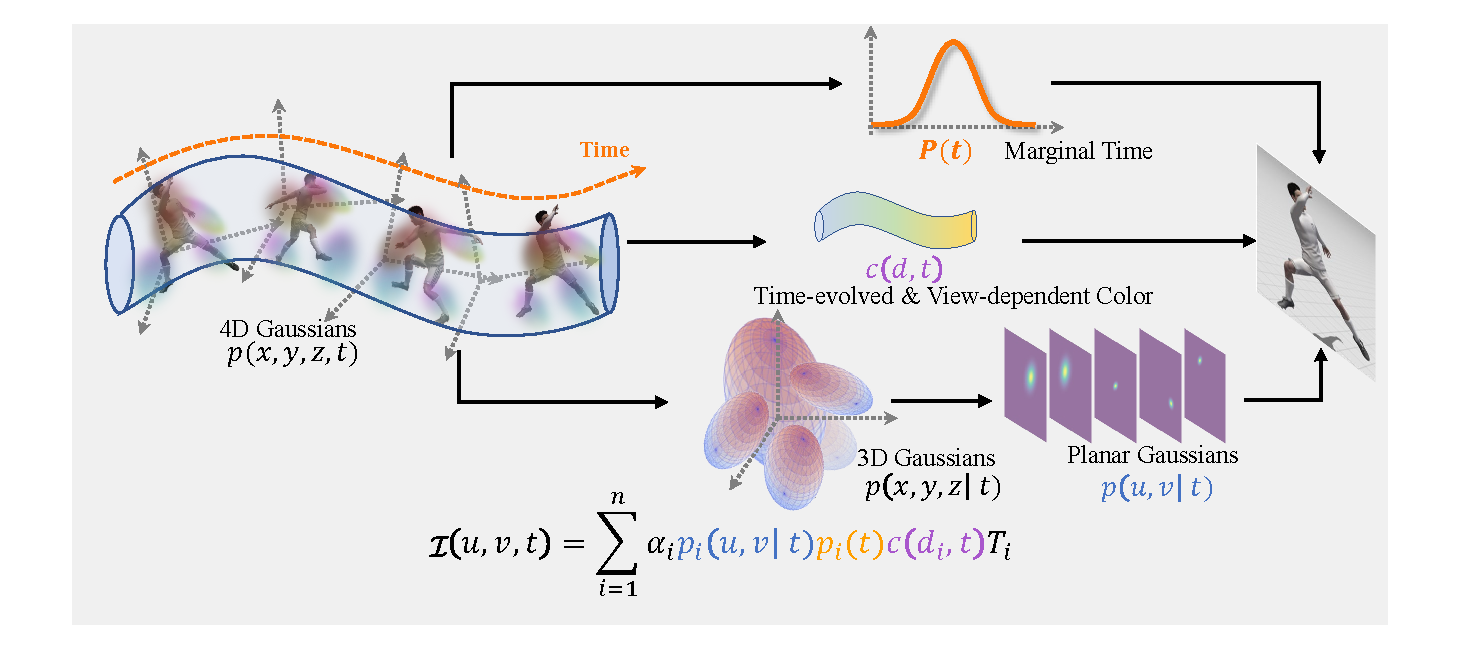
\includegraphics[width=\textwidth]{Grafiken/Fundamentals/pipeline_yang.pdf}
    \caption{The rendering pipeline of the proposed 4DGS method. For a given time \(t\) and view \(I\), each 4D Gaussian is decomposed into a conditional 3D Gaussian and a marginal 1D Gaussian. The conditional 3D Gaussian is then projected onto a 2D splat. Finally, the planar conditional Gaussian, the 1D marginal Gaussian, and the temporally varying, view-dependent color are combined to render the view \(I\) (figure adapted from \cite{yang2023gs4d}).}
    \label{fig:pipeline_real_time_4D}
\end{figure*}

\subsubsection{Extension of the Rendering Equation}

For dynamic scenes, indexing pixels solely by their spatial coordinates \((u,v)\) is insufficient. 
Yang et al.~extend Equation~\ref{eq:projection_3D_gaussians} by an additional timestamp \(t\) to capture the scene dynamics.  
The color \(I(u,v,t)\) of a pixel at time \(t\) is computed by alpha-blending the visible 4D Gaussians:

\begin{align}
I(u,v,t) &= \sum_{i=1}^N p_i(u,v,t) \alpha_i c_i(d) \prod_{j=1}^{i-1} (1 - p_j(u,v,t) \alpha_j)
\end{align}

Here, \(p_i(u,v,t)\) can be further factorized into a conditional probability \(p_i(u,v|t)\) and a marginal probability \(p_i(t)\):

\begin{align}
I(u,v,t) &= \sum_{i=1}^N p_i(t) p_i(u,v|t) \alpha_i c_i(d) \prod_{j=1}^{i-1} (1 - p_j(t) p_j(u,v|t) \alpha_j)
\end{align}

\subsubsection{Scene Representation with 4D Gaussians}

A 4D Gaussian is described by a mean vector \(\mu = (\mu_x, \mu_y, \mu_z, \mu_t)\). 
The definition of the covariance matrix \(\Sigma\) remains identical to the 3DGS formulation~\cite{kerbl3Dgaussians}, factorized via a scaling matrix \(S\) and a rotation matrix \(R\) (cf. Equation~\ref{eq:calc_sigma}).  

The scaling matrix is extended with a temporal scaling factor along the diagonal, resulting in \(S = \mathrm{diag}(s_x, s_y, s_z, s_t)\). 
A rotation in 4D Euclidean space can be constructed from two isotropic rotations, both representable as quaternions. 
This allows anisotropic ellipsoids to rotate freely in space and time.

The left isotropic rotation \(L(q_l)\) and right isotropic rotation \(R(q_r)\) are defined as:

\begin{equation}
R = L(q_l) R(q_r) = 
\begin{pmatrix} 
a & -b & -c & -d \\ 
b & a & -d & c \\
c & d & a & -b \\
d & -c & b & a
\end{pmatrix} 
\begin{pmatrix}
p & -q & -r & -s \\ 
q & p & s & -r \\ 
r & -s & p & q \\ 
s & r & -q & p
\end{pmatrix}.
\label{eq:rotation_matrix}
\end{equation}

\subsubsection{Projection onto the Image Plane}

The conditional 3D Gaussian at a specific time \(p_i(x,y,z|t)\) can now be derived from the properties of the 4D Gaussian:

\begin{align}
\mu_{xyz|t} &= \mu_{1:3} + \Sigma_{1:3,4} \Sigma_{4,4}^{-1} (t - \mu_t) \\
\Sigma_{xyz|t} &= \Sigma_{1:3,1:3} - \Sigma_{1:3,4} \Sigma_{4,4}^{-1} \Sigma_{4,1:3}
\end{align}

After extracting the conditional 3D Gaussians from the 4D representation, the 2D projection can be computed in the same way as for 3DGS.

The marginal distribution \(p_i(t)\) indicates at which times a Gaussian contributes to the scene. 
It can be described by a 1D Gaussian:

\begin{align}
p_i(t) &= \mathcal{N}(t; \mu_4, \Sigma_{4,4})
\end{align}

\subsubsection{Spherical Harmonics for Color Representation}

To model temporal evolution and view-dependent color, spherical harmonics are employed. 
These extend conventional spherical harmonics to account for the temporal dimension. 
The color is represented as a combination of 4D spherical harmonics:

\[
Z_{nlm}(t, \theta, \phi) = \cos\left(\frac{2\pi n}{T} t\right) Y_l^m(\theta, \phi),
\]

where \(Y_l^m\) are the 3D spherical harmonics, \(l\) the degree, \(m\) the order, and \(n\) the Fourier order. 
This enables modeling of temporally varying, view-dependent colors.

% \subsubsection{Evaluation of the Method}

% Compared to previous works, the approach by Yang et al.~\cite{yang2023gs4d} represents a significant advancement, as it enables a consistent representation of dynamic scenes in the space-time continuum while achieving real-time performance. 
% The integration of 4D Gaussians allows for more accurate modeling of temporal dependencies than methods relying solely on 3D representations. 
% However, the original work also highlights limitations: in particular, the increased memory footprint and optimization complexity remain open challenges. 
% Despite these limitations, the method is currently considered a promising approach for photorealistic rendering of dynamic scenes.




\section{Dynamic 3D Gaussians: Tracking by Persistent Dynamic View Synthesis}

One of the foundational works for dynamic Gaussian Splatting is the method proposed by Luiten et al.~\cite{luiten2024dynamic}, which introduces \textit{Dynamic 3D Gaussians} (D3DGS) for representing and tracking dynamic scenes. 
This method forms the basis for the dynamic object reconstruction component of the pipeline developed in this work. 
The following section provides a detailed overview of its representation, physical regularization, and optimization strategy.

\subsubsection{Scene Representation}

In contrast to approaches that model space and time within a shared continuum, D3DGS explicitly tracks Gaussian primitives over time. 
While 3DGS treats Gaussians as static entities in three-dimensional space, D3DGS extends this framework by allowing their positions and orientations to vary across frames. 
Intrinsic properties such as color, opacity, and scale remain fixed, resulting in a representation where Gaussians behave like physical particles undergoing rigid-body motion. 
The method maintains a fixed number of Gaussians per scene rather than dynamically creating or deactivating them over time. 
This consistency facilitates compositional workflows, as objects can be represented and manipulated uniformly across scenes. 
To ensure physically plausible and temporally coherent motion, Luiten et al. augment the model with several regularization terms that encode physical priors.

\begin{figure*}[ht]
    \centering
    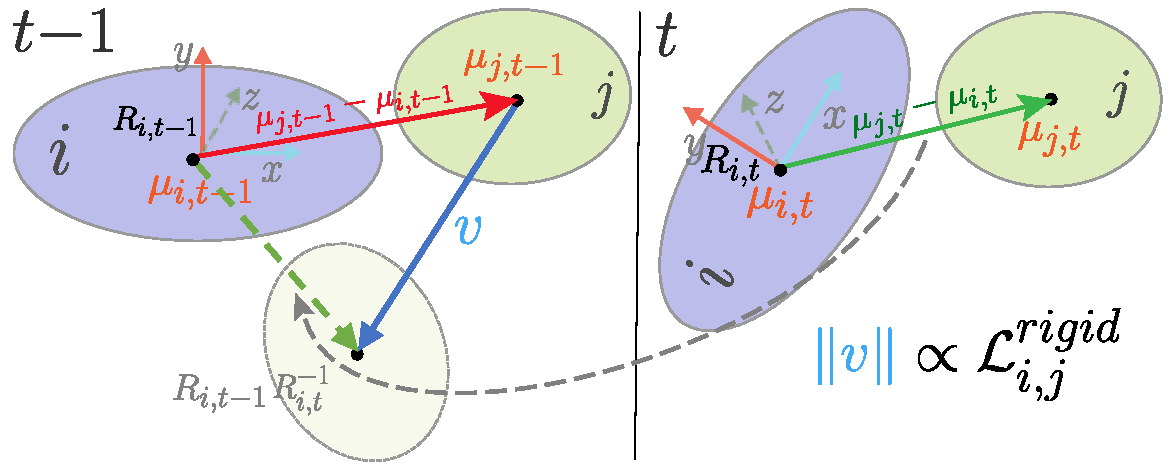
\includegraphics[width=\textwidth]{Grafiken/Fundamentals/loss_fig_luiten.pdf}
    \caption{Schematic illustration of the local rotation similarity loss in D3DGS~\cite{luiten2024dynamic}.}
    \label{fig:loss_fig_luiten}
\end{figure*}

\subsubsection{Physical Regularization}

The physical regularization ensures that local structures move consistently and undergo realistic motion patterns. 
Three principal loss terms are introduced to enforce these constraints.

\paragraph{Local Rigidity Loss}

The rigidity loss enforces that neighboring Gaussians exhibit motion consistent with a local rigid-body transformation. 
For each Gaussian \(i\), its neighbors \(j\) across two consecutive time steps should follow a similar transformation (see Fig.~\ref{fig:loss_fig_luiten}). 
The loss is defined as:
\begin{align}
\rigidloss = \frac{1}{k|S|} \sum_{i \in S} \sum_{j \in \text{k-nn}} w_{i,j} \|(\mu_{j,t-1} - \mu_{i,t-1}) - R_{i,t-1} R_{i,t}^{-1} (\mu_{j,t} - \mu_{i,t})\|^2,
\end{align}
where the weighting factor \(w_{i,j}\) depends on the spatial proximity of two Gaussians in the initial configuration:
\begin{align}
w_{i,j} = \exp \left( -\lambda_w \|\mu_{j,0} - \mu_{i,0}\|^2 \right).
\end{align}
This loss preserves the relative structure of local neighborhoods over time.

\paragraph{Local Rotation Similarity Loss}

In addition to translation, the rotation of neighboring Gaussians should remain consistent. 
To achieve this, a rotation similarity loss measures the difference between the quaternions representing the local motion:
\begin{align}
\rotloss = \frac{1}{k|S|} \sum_{i \in S} \sum_{j \in \text{k-nn}} w_{i,j} \|q_{j,t} q_{j,t-1}^{-1} - q_{i,t} q_{i,t-1}^{-1}\|^2.
\end{align}
This encourages spatially coherent rotational motion across neighboring Gaussians.

\paragraph{Isometry Loss}

The isometry loss stabilizes the distances between Gaussians over time, preventing local neighborhoods from deforming excessively. 
It is defined as:
\begin{align}
\isoloss = \frac{1}{k|S|} \sum_{i \in S} \sum_{j \in \text{k-nn}} w_{i,j} \left| \|\mu_{j,0} - \mu_{i,0}\| - \|\mu_{j,t} - \mu_{i,t}\| \right|.
\end{align}
Compared to the more restrictive rigidity loss, this term acts as a softer constraint, allowing moderate flexibility while maintaining approximately constant inter-Gaussian distances.

\subsubsection{Optimization}

Optimization follows the same principle as static 3DGS and relies on the image reconstruction loss defined in Equation~\ref{eq:loss_GS}. 
Training proceeds sequentially over time steps, leading to a linear increase in computation time with sequence length. 
A major limitation of this formulation is its reliance on dense multi-view supervision: 
if certain viewpoints are missing, Gaussians that become occluded or leave the field of view can no longer be reliably tracked, reducing robustness in scenes with partial visibility.
